\begin{figure}[htbp]
  \centering
  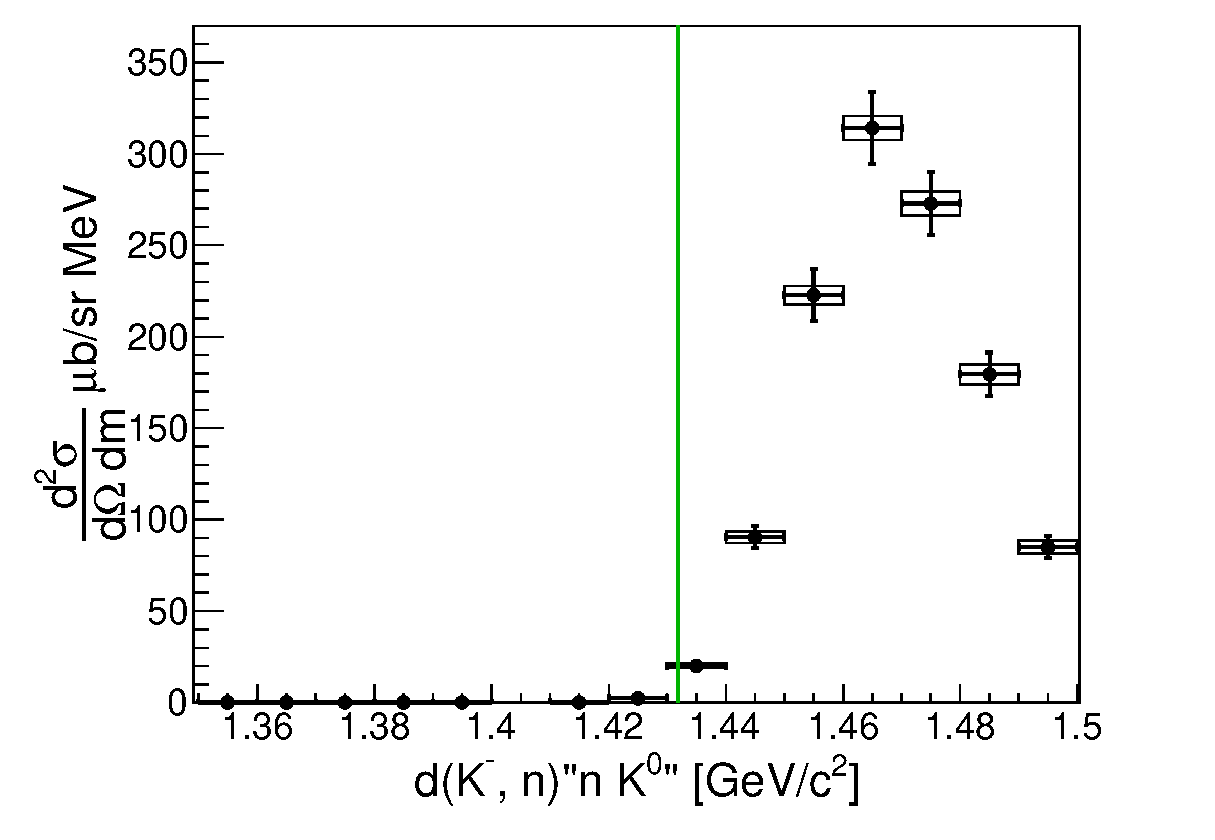
\includegraphics[width=6cm]{../pic/Dron/K0_ana/K0_CS.eps}
  \caption{
    This figure shows the cross section of $d(K^-, n)"n K^0"$.
    The box represents the statistical error, and the error bar represents the root mean squares of the conversion factor added to it.
    The green vertical lines indicates $\bar{K}N$ threshold.
  }
  \label{fig:nK0_CS}
\end{figure}

\begin{figure}[htbp]
  \centering
  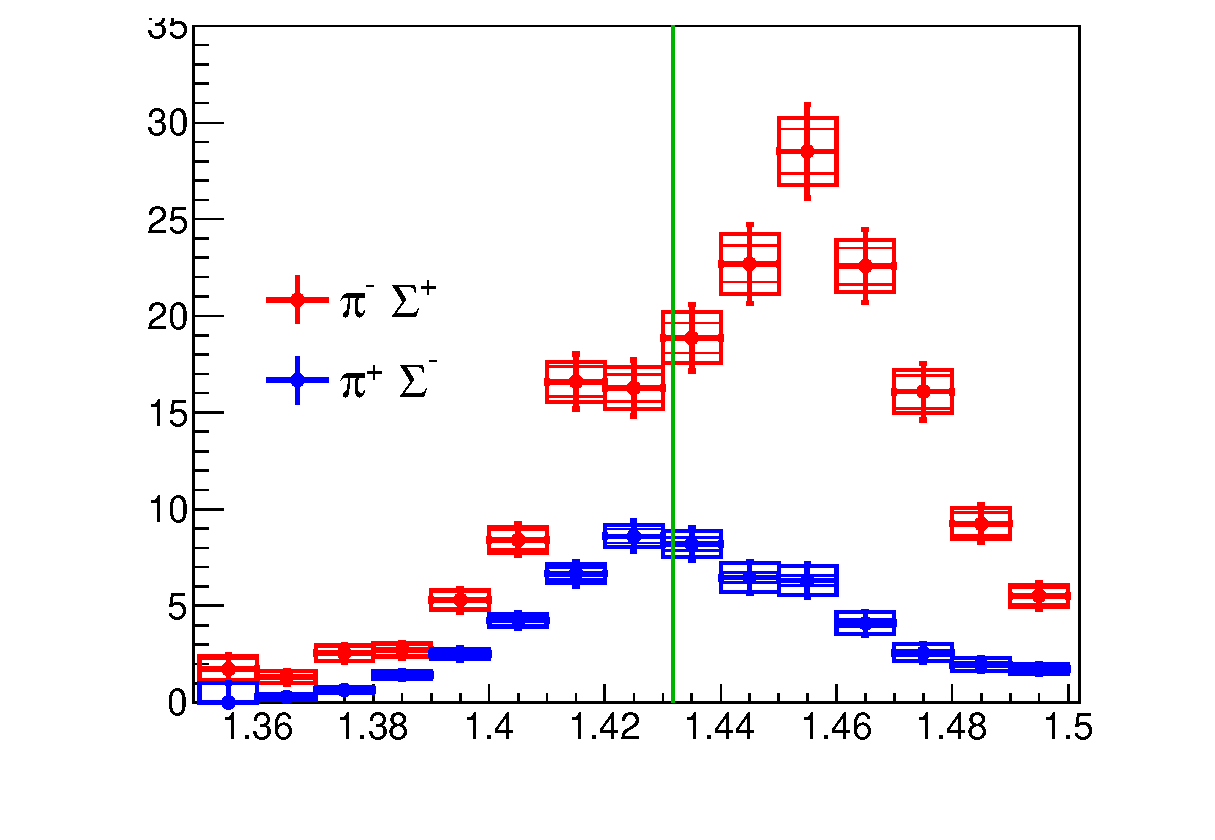
\includegraphics[width=6cm]{../pic/Dron/KN_ana/ChargeCS.eps}
  \caption{
    The red figure and blue figure shows about $d(K^-, n)"\pi^+\Sigma^-"$ and $d(K^-, n)"\pi^-\Sigma^+"$, respectively.
    The inner frame (thin line), outer frame (thick line), and error bars represent the addition of statistical errors, fitting errors, and conversion errors, which were calculated by root-mean-square.
    The green vertical lines indicates $\bar{K}N$ threshold.
  }
  \label{fig:ChargeCS}
\end{figure}

\begin{figure}[htbp]
  \centering
  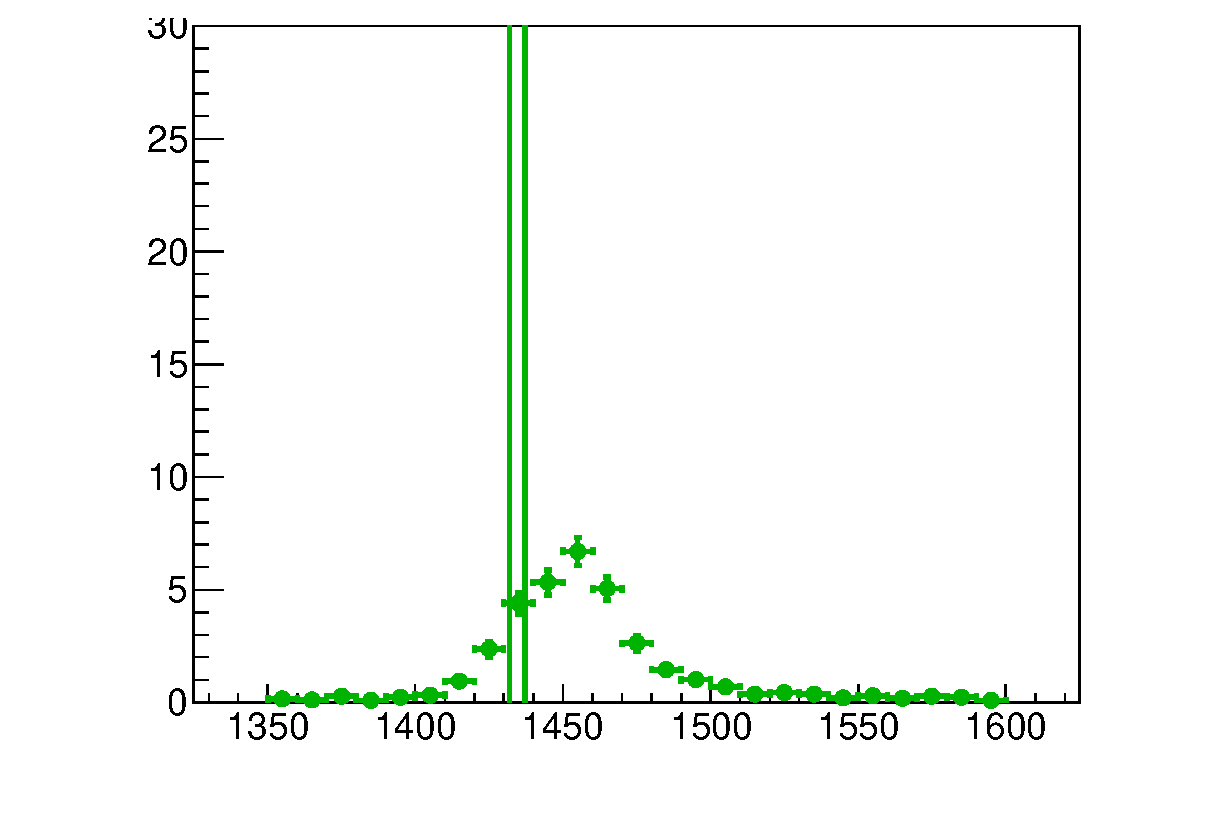
\includegraphics[width=6cm]{../pic/Dron/KP_ana/pimS0_CS.eps}
  \caption{
    This figure shows the cross section of $d(K^-, p)"\pi^- \Sigma^0"$.
    The box represents the statistical error, and the error bar represents the root mean squares of the conversion factor added to it.
    The green vertical lines indicates $\bar{K}N$ threshold.
  }
  \label{fig:pimS0_CS}
\end{figure}
